\documentclass[journal,onecolumn]{IEEEtran}
\usepackage[T1]{fontenc}
\usepackage{amsmath}
\usepackage{graphicx}
\usepackage{booktabs}
\usepackage[hidelinks]{hyperref}
\graphicspath{{figures/}}

\newcommand{\AP}{\mathrm{AP}_{0.05}}
\newcommand{\Fmain}{\mathrm{F1}_{0.975}}
\newcommand{\Falt}{\mathrm{F1}_{0.95}}
\renewcommand{\thetable}{S\arabic{table}}
\renewcommand{\thefigure}{S\arabic{figure}}

\title{Supplementary Material}
\author{Ignacio~Martin-Salinas, Jose~A.~Belloch, Adri\'an~Amor-Mart\'in, Pablo~Zumel, and~Cristina~Fernandez}

\begin{document}
\maketitle
\suppressfloats[t]

\begin{center}
\emph{Detecting Component Degradation Under Variable Load From Buck Converter Frequency Responses}
\end{center}

\section*{Detailed Benchmark Results}

Tables~\ref{tab:variable_load_benchmark}--\ref{tab:lofo_generalization} provide the full metrics for the benchmarks, ablations, and robustness tests summarized in the manuscript. The subscripts of $\Fmain$ and $\Falt$ denote healthy validation quantiles, and $\AP$ is average precision adjusted to an assumed anomaly prevalence of $5\%$.

\begin{table*}[t]
\centering
\caption{Zero-anomaly-label (\texttt{p97.5}) anomaly detection performance on the variable-load benchmark (\texttt{dataset\_02}, $R_{\mathrm{out}} \in [2, 8]\,\Omega$). Deep models report mean $\pm$ SD over 10 random seeds; \texttt{Supervised GBM Oracle} uses 90 labeled validation anomalies solely as a supervised reference.}
\label{tab:variable_load_benchmark}
\resizebox{\textwidth}{!}{%
\begin{tabular}{lcccccrrrrrr}
\toprule
Detector / Paradigm & Uses Fault Labels? & $\mathrm{F1}_{\mathrm{p97.5}}$ & $\mathrm{F1}_{\mathrm{p95}}$ & $\mathrm{PR\text{-}AUC}_{\pi=0.05}$ & $\mathrm{ROC\text{-}AUC}$ & $C_{\mathrm{out}}$ Rec. & $\mathrm{ESR}_C$ Rec. & $L_{\mathrm{out}}$ Rec. & $\mathrm{ESR}_L$ Rec. & $R_{\mathrm{ds},1}$ Rec. & Multi Rec. \\
\midrule
\texttt{One-Class SVM (RBF)} & No & 0.6892 & 0.6951 & 0.5434 & 0.7730 & 91.3\% & 3.6\% & 90.9\% & 4.8\% & 0.0\% & 71.1\% \\
\texttt{Raw k-NN (k=5)} & No & 0.7112 & 0.7087 & 0.6268 & 0.8716 & 91.3\% & 3.6\% & 90.9\% & 4.8\% & 0.0\% & 76.3\% \\
\texttt{Mahalanobis (Ridge 1e-6)} & No & 0.7638 & 0.8274 & 0.7086 & 0.9246 & 91.3\% & 21.4\% & 90.9\% & 4.8\% & 5.3\% & 84.5\% \\
\texttt{Isolation Forest (200)} & No & 0.8347 & 0.8962 & 0.7289 & 0.9293 & 100.0\% & 60.7\% & 95.5\% & 19.0\% & 10.5\% & 89.7\% \\
\texttt{Mahalanobis (Ledoit-Wolf)} & No & 0.8992 & 0.9196 & 0.7874 & 0.9582 & 100.0\% & 71.4\% & 95.5\% & 66.7\% & 15.8\% & 95.9\% \\
\texttt{PCA (99\% Var., d=4)} & No & 0.7493 & 0.7608 & 0.6602 & 0.8993 & 95.7\% & 14.3\% & 90.9\% & 9.5\% & 0.0\% & 81.4\% \\
\texttt{PCA (Oracle d=10, Clean)} & Oracle $d$ & 0.9347 & 0.9453 & 0.8538 & 0.9703 & 95.7\% & 89.3\% & 95.5\% & 90.5\% & 21.1\% & 97.9\% \\
\textbf{\texttt{CARLA-Transformer (SSA)}} & \textbf{No} & \textbf{0.9417 $\pm$ 0.0128} & \textbf{0.9433 $\pm$ 0.0095} & \textbf{0.9126 $\pm$ 0.0308} & \textbf{0.9740 $\pm$ 0.0064} & \textbf{100.0\%} & \textbf{89.6\%} & \textbf{91.8\%} & \textbf{92.4\%} & \textbf{36.3\%} & \textbf{97.4\%} \\
\textit{\texttt{Supervised GBM Oracle}} & \textit{Yes (90 faults)} & \textit{0.9340} & \textit{---} & \textit{0.9322} & \textit{0.9797} & \textit{87.0\%} & \textit{100.0\%} & \textit{90.9\%} & \textit{81.0\%} & \textit{15.8\%} & \textit{99.0\%} \\
\bottomrule
\end{tabular}%
}
\end{table*}

\begin{table*}[!t]
\centering
\caption{Paired Transformer ablation on the variable-load benchmark over ten seeds.}
\label{tab:10seed_ablation}
\footnotesize
\setlength{\tabcolsep}{5pt}
\renewcommand{\arraystretch}{1.17}
\begin{tabular*}{\textwidth}{@{\extracolsep{\fill}}lccc@{}}
\toprule
Training and scoring & $\Fmain$ & $\AP$ & ROC AUC \\
\midrule
Reconstruction error & $0.7540 \pm 0.0111$ & $0.6640 \pm 0.0153$ & $0.9033 \pm 0.0129$ \\
Reconstruction latent $k$-NN & $0.7090 \pm 0.0067$ & $0.6129 \pm 0.0053$ & $0.8190 \pm 0.0114$ \\
Heuristic negatives & $0.6868 \pm 0.0281$ & $0.5272 \pm 0.0529$ & $0.8344 \pm 0.0224$ \\
SSA negatives & $0.9417 \pm 0.0128$ & $0.9126 \pm 0.0308$ & $0.9740 \pm 0.0064$ \\
\bottomrule
\end{tabular*}
\par\smallskip
\textit{Recall at the 97.5th percentile (\%)}\par\smallskip
\begin{tabular*}{\textwidth}{@{\extracolsep{\fill}}lccccc@{}}
\toprule
Training and scoring & Passive & $\mathrm{ESR}_C$ & $\mathrm{ESR}_L$ & $R_{\mathrm{ds},1}$ & $\Delta$F1 \\
\midrule
Reconstruction error & $51.7 \pm 2.0$ & $13.2 \pm 2.9$ & $9.5 \pm 6.3$ & $3.2 \pm 2.7$ & $+0.1876$ \\
Reconstruction latent $k$-NN & $45.4 \pm 0.7$ & $3.6 \pm 0.0$ & $4.8 \pm 0.0$ & $1.1 \pm 2.2$ & $+0.2327$ \\
Heuristic negatives & $45.7 \pm 3.8$ & $17.1 \pm 4.4$ & $5.2 \pm 3.5$ & $6.8 \pm 3.6$ & $+0.2548$ \\
SSA negatives & $93.3 \pm 2.2$ & $89.6 \pm 7.2$ & $92.4 \pm 4.0$ & $36.3 \pm 10.4$ & --- \\
\bottomrule
\end{tabular*}
\par\smallskip\parbox{\textwidth}{Values are mean $\pm$ SD. Passive recall pools the four passive single-fault strata. $\Delta$F1 is the mean paired improvement with SSA negatives. Each paired comparison gives $p=0.00195$ (unadjusted).}
\end{table*}

\begin{table*}[!ht]
\centering
\caption{Encoder comparisons with the same SSA-ratio augmentation on the variable-load benchmark.}
\label{tab:encoder_backbones}
\footnotesize
\setlength{\tabcolsep}{3pt}
\renewcommand{\arraystretch}{1.17}
\begin{tabular*}{\textwidth}{@{\extracolsep{\fill}}lccccccc@{}}
\toprule
& \multicolumn{4}{c}{Aggregate metrics} & \multicolumn{3}{c}{Clean recall (\%)} \\
\cmidrule(lr){2-5}\cmidrule(l){6-8}
Encoder & Clean $\Fmain$ & Noisy $\Fmain$ & $\AP$ & ROC AUC & $\mathrm{ESR}_C$ & $\mathrm{ESR}_L$ & $R_{\mathrm{ds},1}$ \\
\midrule
Transformer & $0.9447 \pm 0.0133$ & $0.9303 \pm 0.0087$ & $0.9195 \pm 0.0283$ & $0.9733 \pm 0.0069$ & $90.0 \pm 9.2$ & $94.3 \pm 2.1$ & $38.9 \pm 8.0$ \\
LSTM & $0.8611 \pm 0.0144$ & $0.8557 \pm 0.0165$ & $0.8053 \pm 0.0100$ & $0.9254 \pm 0.0033$ & $84.3 \pm 11.5$ & $24.8 \pm 4.0$ & $7.4 \pm 4.7$ \\
1-D convolution & $0.8426 \pm 0.0238$ & $0.7451 \pm 0.0165$ & $0.7440 \pm 0.0099$ & $0.9188 \pm 0.0083$ & $53.6 \pm 13.4$ & $50.5 \pm 19.2$ & $3.2 \pm 4.7$ \\
MLP & $0.7739 \pm 0.0210$ & $0.7506 \pm 0.0207$ & $0.7227 \pm 0.0322$ & $0.9095 \pm 0.0118$ & $30.0 \pm 10.6$ & $17.1 \pm 12.0$ & $6.3 \pm 6.9$ \\
GRU & \shortstack{$0.5988 \pm 0.3207$\\{\scriptsize [0.8164]}} & \shortstack{$0.6021 \pm 0.2965$\\{\scriptsize [0.7910]}} & \shortstack{$0.5147 \pm 0.3052$\\{\scriptsize [0.6958]}} & \shortstack{$0.7904 \pm 0.1128$\\{\scriptsize [0.8632]}} & $60.7 \pm 52.2$ & $7.6 \pm 5.4$ & $3.2 \pm 4.7$ \\
\bottomrule
\end{tabular*}
\par\smallskip\parbox{\textwidth}{Values are mean $\pm$ SD over five seeds. Brackets give the GRU medians. The noisy condition uses $0.15\,\mathrm{dB}$ magnitude and $0.75^\circ$ phase jitter.}
\end{table*}

\begin{table*}[t]
\centering
\caption{Representation-versus-scorer control matrix on {\upshape\ttfamily dataset\_02} (10 seeds, zero-label {\upshape\ttfamily p97.5} F1 and $\mathrm{PR\text{-}AUC}_{\pi=0.05}$).}
\label{tab:representation_vs_scorer}
\resizebox{\textwidth}{!}{%
\begin{tabular}{lcccccc}
\toprule
Learned Representation (10 Seeds) & \texttt{k-NN (k=5)} $\mathrm{F1}_{\mathrm{p97.5}}$ & \texttt{Ledoit-Wolf} $\mathrm{F1}_{\mathrm{p97.5}}$ & \texttt{PCA (d=5)} $\mathrm{F1}_{\mathrm{p97.5}}$ & \texttt{PCA (d=10)} $\mathrm{F1}_{\mathrm{p97.5}}$ & \texttt{k-NN (k=5)} $\mathrm{PR\text{-}AUC}_{\pi=0.05}$ & \texttt{Ledoit-Wolf} $\mathrm{PR\text{-}AUC}_{\pi=0.05}$ \\
\midrule
\texttt{AE-Transformer} ($\mathbf{h}$, $w_c=0$) & 0.7090 $\pm$ 0.0067 & 0.7671 $\pm$ 0.0289 & 0.8293 $\pm$ 0.0597 & 0.9373 $\pm$ 0.0208 & 0.6129 $\pm$ 0.0053 & 0.6662 $\pm$ 0.0324 \\
\texttt{CARLA (Heuristic)} ($\mathbf{z}$) & 0.6868 $\pm$ 0.0281 & 0.8042 $\pm$ 0.0247 & 0.6674 $\pm$ 0.0606 & 0.7343 $\pm$ 0.0425 & 0.5271 $\pm$ 0.0530 & 0.6902 $\pm$ 0.0470 \\
\textbf{\texttt{CARLA (SSA)} Latent ($\mathbf{h}$)} & \textbf{0.9296 $\pm$ 0.0203} & \textbf{0.9421 $\pm$ 0.0037} & \textbf{0.9502 $\pm$ 0.0036} & \textbf{0.9204 $\pm$ 0.0188} & \textbf{0.8898 $\pm$ 0.0182} & \textbf{0.8620 $\pm$ 0.0064} \\
\textbf{\texttt{CARLA (SSA)} Projection ($\mathbf{z}$)} & \textbf{0.9415 $\pm$ 0.0125} & \textbf{0.9504 $\pm$ 0.0109} & \textbf{0.9351 $\pm$ 0.0129} & \textbf{0.9474 $\pm$ 0.0121} & \textbf{0.9126 $\pm$ 0.0304} & \textbf{0.9188 $\pm$ 0.0237} \\
\bottomrule
\end{tabular}%
}
\end{table*}

\begin{table*}[t]
\centering
\caption{Parametric FRA instrument-noise robustness sweep on {\upshape\ttfamily dataset\_02} across seven polar jitter levels $(\sigma_{\mathrm{dB}},\, \sigma_{\mathrm{deg}} = 5\sigma_{\mathrm{dB}})$ under zero-label {\upshape\ttfamily p97.5} calibration.}
\label{tab:fra_noise_sweep}
\resizebox{\textwidth}{!}{%
\begin{tabular}{lccccccc}
\toprule
Detector (Zero-Label \texttt{p97.5}) & $0.00\,\mathrm{dB}$ ($0.00^\circ$) & $0.05\,\mathrm{dB}$ ($0.25^\circ$) & $0.10\,\mathrm{dB}$ ($0.50^\circ$) & $0.15\,\mathrm{dB}$ ($0.75^\circ$) & $0.25\,\mathrm{dB}$ ($1.25^\circ$) & $0.40\,\mathrm{dB}$ ($2.00^\circ$) & $0.60\,\mathrm{dB}$ ($3.00^\circ$) \\
\midrule
\textbf{\texttt{CARLA-Transformer (SSA)} (10 seeds)} & \textbf{0.9417 $\pm$ 0.0128} & \textbf{0.9414 $\pm$ 0.0117} & \textbf{0.9313 $\pm$ 0.0108} & \textbf{0.9160 $\pm$ 0.0138} & \textbf{0.9025 $\pm$ 0.0199} & \textbf{0.8304 $\pm$ 0.0375} & \textbf{0.7695 $\pm$ 0.0240} \\
\texttt{PCA Reconstruction (Oracle d=8)} & \textbf{0.9584} & 0.9417 & 0.8923 & 0.7967 & 0.6869 & 0.5245 & 0.4509 \\
\texttt{PCA Reconstruction (Oracle d=10)} & 0.9347 & 0.8682 & 0.7331 & 0.6478 & 0.5492 & 0.4328 & 0.3615 \\
\texttt{PCA (d=8, Re-fit on Noisy Train)} & 0.9584 & 0.9443 & 0.8951 & 0.8177 & 0.7337 & 0.6852 & 0.6770 \\
\texttt{Mahalanobis (Ledoit-Wolf)} & 0.8992 & 0.8783 & 0.8122 & 0.7240 & 0.6749 & 0.5646 & 0.4509 \\
\texttt{Raw k-NN (k=5)} & 0.7112 & 0.7112 & 0.7112 & 0.7112 & 0.7091 & 0.7073 & 0.6991 \\
\bottomrule
\end{tabular}%
}
\vspace{2pt}\par\footnotesize\textit{Note:} On the primary matched 0.15 dB calibration realization (Fig. 6a), CARLA-Transformer (SSA) achieves F1 = 0.9284 $\pm$ 0.0154.
\end{table*}

\begin{table*}[!ht]
\centering
\caption{Leave-one-fault-out evaluation of the SSA-ratio Transformer over five seeds.}
\label{tab:lofo_generalization}
\footnotesize
\setlength{\tabcolsep}{5pt}
\renewcommand{\arraystretch}{1.17}
\begin{tabular*}{\textwidth}{@{\extracolsep{\fill}}lccccc@{}}
\toprule
Omitted mode & $n$ & Held-out ROC AUC & Held-out recall (\%) & Included recall (\%) & Overall $\Fmain$ \\
\midrule
$C_{\mathrm{out}}$ & $23$ & \shortstack{$0.9989 \pm 0.0008$\\{\scriptsize [0.9991, 0.0009]}} & \shortstack{$99.1 \pm 1.9$\\{\scriptsize [100.0, 0.0]}} & $100.0 \pm 0.0$ & $0.9482 \pm 0.0094$ \\
$L_{\mathrm{out}}$ & $22$ & \shortstack{$0.9911 \pm 0.0027$\\{\scriptsize [0.9905, 0.0014]}} & \shortstack{$93.6 \pm 2.5$\\{\scriptsize [95.5, 4.5]}} & $91.8 \pm 2.0$ & $0.9473 \pm 0.0071$ \\
$\mathrm{ESR}_C$ & $28$ & \shortstack{$0.9715 \pm 0.0525$\\{\scriptsize [0.9939, 0.0079]}} & \shortstack{$82.9 \pm 24.7$\\{\scriptsize [92.9, 3.6]}} & $90.0 \pm 9.2$ & $0.9106 \pm 0.0687$ \\
$\mathrm{ESR}_L$ & $21$ & \shortstack{$0.9470 \pm 0.0717$\\{\scriptsize [0.9705, 0.0214]}} & \shortstack{$75.2 \pm 31.5$\\{\scriptsize [90.5, 4.8]}} & $94.3 \pm 2.1$ & $0.9087 \pm 0.0749$ \\
$R_{\mathrm{ds},1}$ & $19$ & \shortstack{$0.7466 \pm 0.0563$\\{\scriptsize [0.7684, 0.0442]}} & \shortstack{$30.5 \pm 13.6$\\{\scriptsize [31.6, 10.5]}} & $38.9 \pm 8.0$ & $0.9177 \pm 0.0524$ \\
\bottomrule
\end{tabular*}
\par\smallskip\parbox{\textwidth}{Values are mean $\pm$ SD, with [median, interquartile range] where indicated. Recall is measured at the healthy validation 97.5th percentile. Included recall is the reference obtained with all five modes in augmentation.}
\end{table*}


\clearpage
\section*{Frequency Dependence of Attention and Score Sensitivity}

We compare mean attention assigned to each key frequency and the norm of the anomaly-score gradient with respect to the two standardized channels at that frequency. For the reconstruction-only control the score is nearest-neighbor distance in the encoder representation. The contrastive models use their normalized projections. The gradient norms are averaged over sweeps and normalized by the total across frequencies for each run. Attention weights are reported as a complementary description of the model.

\begin{figure}[!h]
\centering
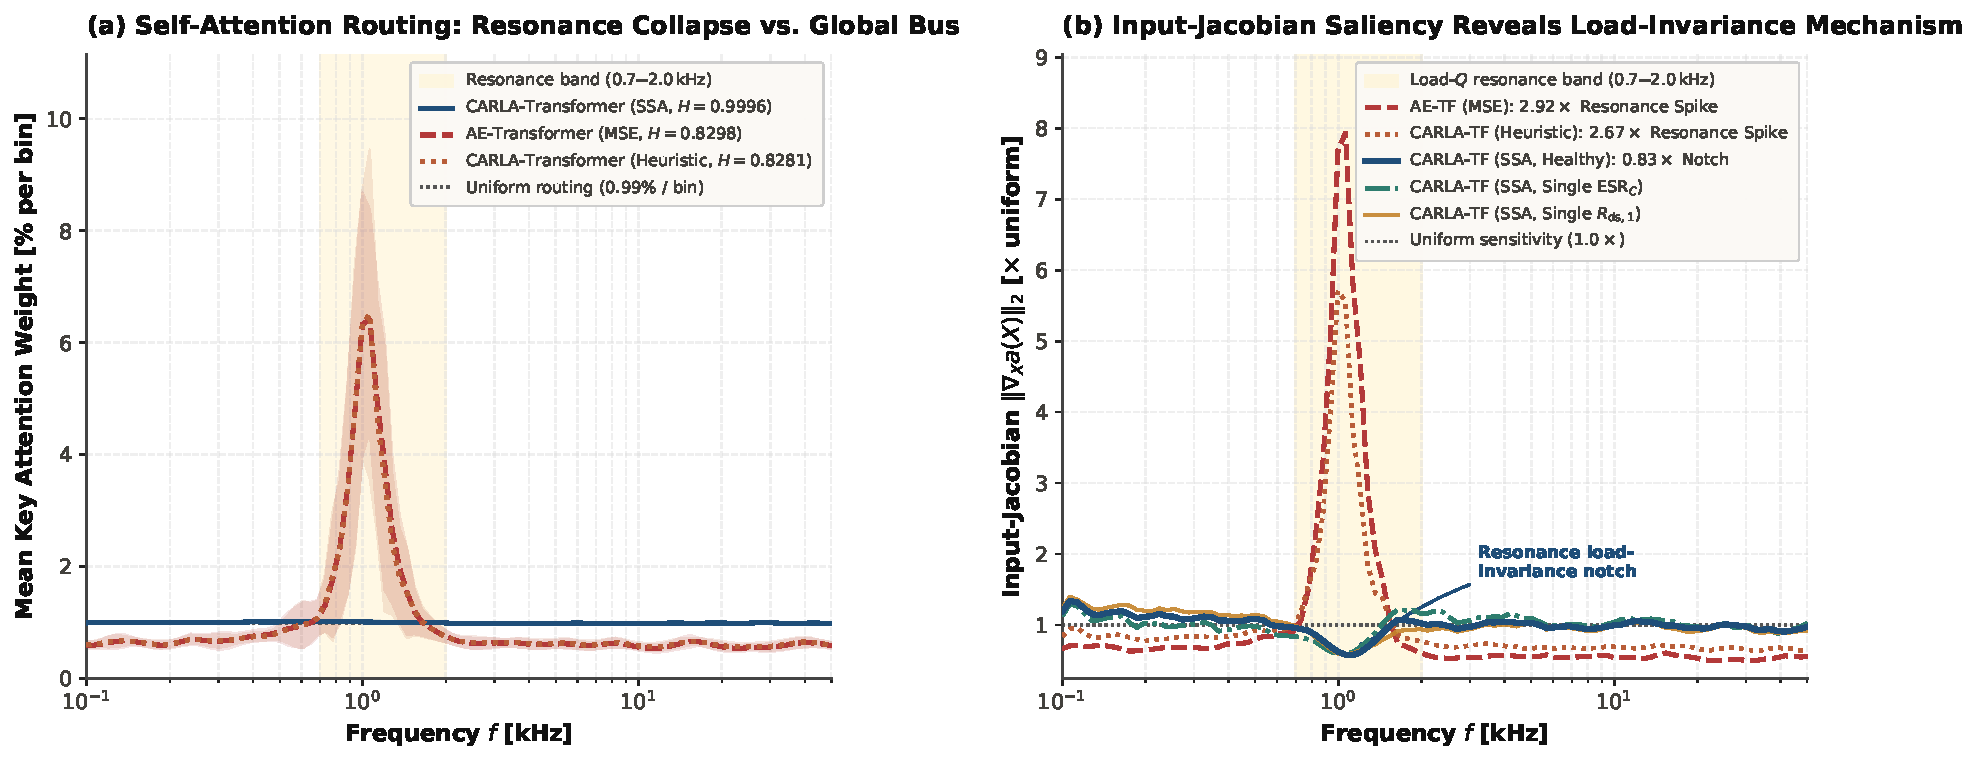
\includegraphics[width=\textwidth]{fig09_attention_and_jacobian_saliency.pdf}
\caption{Attention and score sensitivity on the variable-load benchmark. (a) Mean attention weight per key frequency. The uniform reference is $100/101\%$ per bin, and $H$ is normalized Shannon entropy. (b) Norm of the score gradient per frequency, shown relative to uniform sensitivity. The shaded regions mark the $0.7$--$2.0\,\mathrm{kHz}$ resonance band.}
\label{fig:fig09}
\end{figure}

The reconstruction-only and heuristic-negative Transformers concentrate mean attention near $1.01\,\mathrm{kHz}$, with normalized entropies of $0.8298\pm0.0421$ and $0.8281\pm0.0423$, respectively. Mean attention is nearly uniform for the SSA-ratio Transformer ($0.9996\pm0.0002$) [Fig.~\ref{fig:fig09}(a)]. In the resonance band, the corresponding normalized gradient sensitivities are $2.92$ and $2.67$ for the two controls, compared with $0.833\pm0.086$ for the SSA-ratio model on healthy sweeps [Fig.~\ref{fig:fig09}(b)]. The SSA-ratio model shows relatively higher low-frequency sensitivity for inductor ESR and high-side switch faults, consistent with the gain changes described by the averaged converter model in the manuscript. These observations characterize local model sensitivity. Establishing invariance to load would require perturbations along measured or simulated load trajectories.

\end{document}
